\sectionframe{What is Period-adding?}
\section{What is Period-adding?}

\begin{frame}{Period-adding}
	\vspace{-1em}
	\begin{columns}
		\begin{column}{.5 \textwidth}
			\begin{figure}
				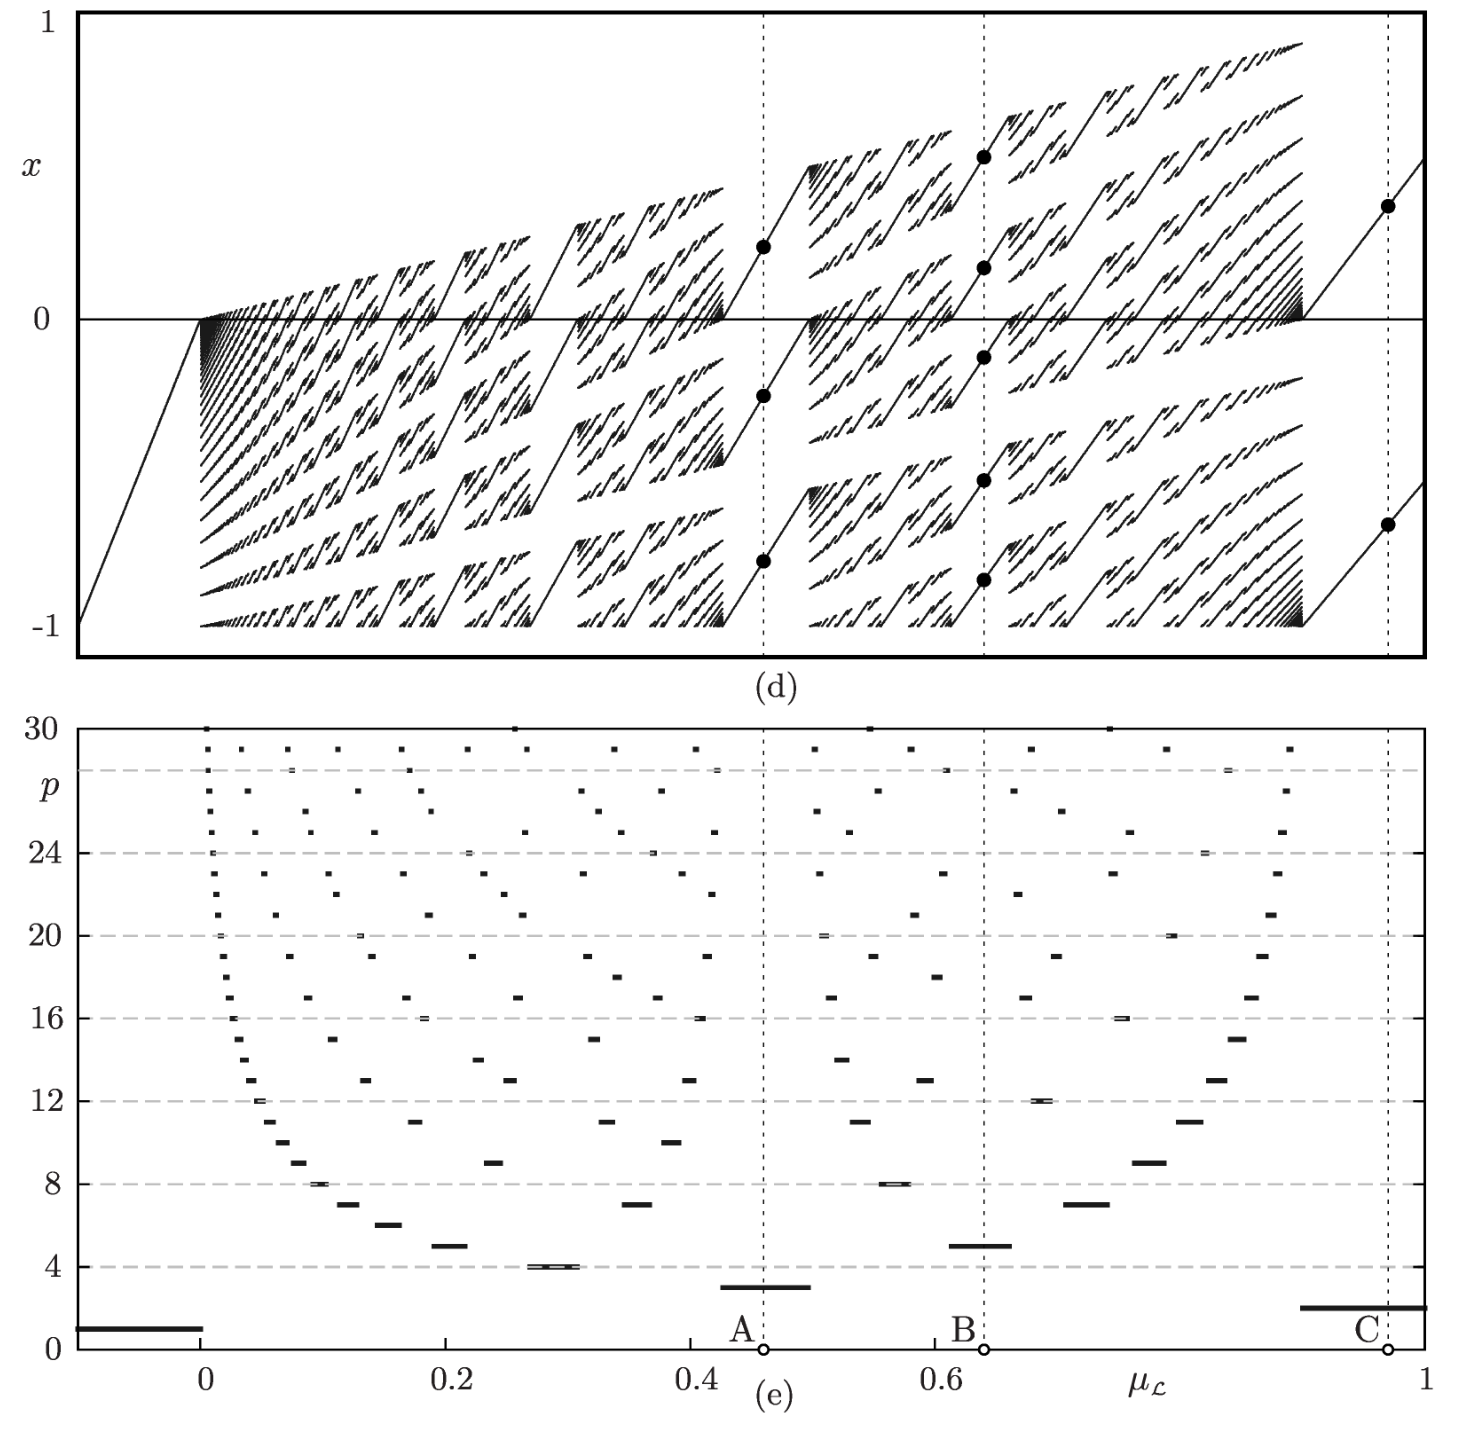
\includegraphics[width=.8 \textwidth]{Figs/PeriodAddingDiagrams_Slides.png}
			\end{figure}
		\end{column}
		\begin{column}{.5 \textwidth}
			\only<2->{
				\begin{figure}
					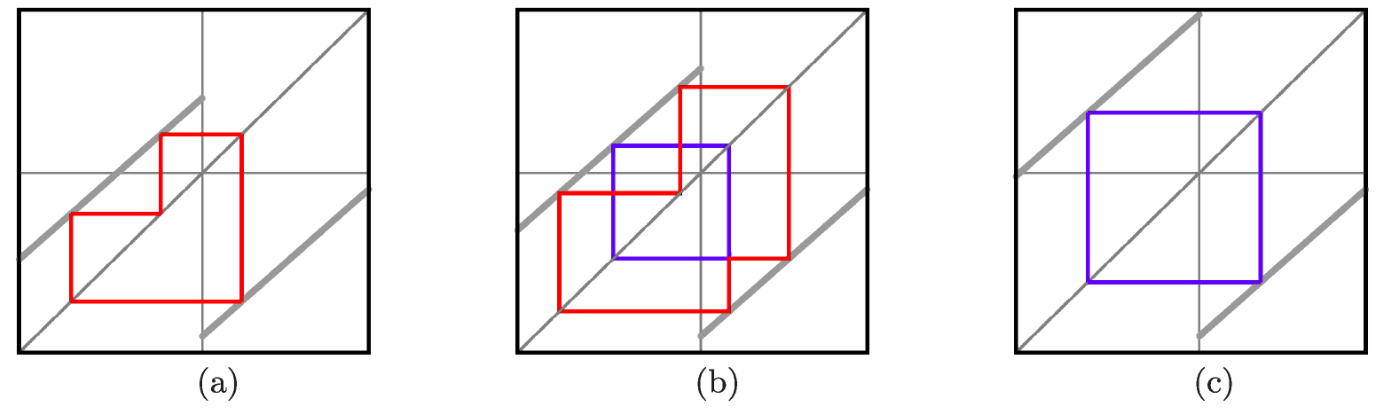
\includegraphics[width=\textwidth]{Figs/PeriodAddingCobwebs_Slides.png}
				\end{figure}
				\pause
				\pause
				\begin{itemize}
					\item In the middle of two cycles with periods $a$ and $b$:
					\item A cycle with period $a + b$
					\item How are these cycles organized?
					\item Are there rules for their symbolic sequences?
				\end{itemize}
			}
		\end{column}
	\end{columns}
\end{frame}

\begin{frame}{A Seemingly Unrelated Concept}
	Farey-sequences
	\begin{itemize}
		\item First discovered by Charles Haros in 1802
		\item Rediscovered by and named after John Farey in 1816 \pause
		\item Also used by Louis-Achille Brocot, a french clock-maker
		\item Dealing with gear ratios \pause
		\item Possible connection: Gears have a descrete number of teeth and cycles have a discrete number of points
	\end{itemize}
	\todo{Expand on connection?}
\end{frame}

\begin{frame}{Farey-sequences}
	\vspace{-1em}
	\begin{definition}[Farey-sequences]
		The Farey-sequence $\F^m$ of order $m$ is defined as the set of irreducible fractions in the closed interval $[0, 1]$
		with denominators not larger than $m$, listed in increasing order.
	\end{definition}
	\pause
	\begin{itemize}
		\item $\F^1 = \left\{ \frac{0}{1}, \frac{1}{1} \right\}$ \vspace{.1em}
		\item $\F^2 = \left\{ \frac{0}{1}, \frac{1}{2}, \frac{1}{1} \right\}$ \vspace{.1em}
		\item $\F^3 = \left\{ \frac{0}{1}, \frac{1}{3}, \frac{1}{2}, \frac{2}{3}, \frac{1}{1} \right\}$
	\end{itemize}
	\pause
	\begin{theorem}[Farey-addition]
		Let $\frac{a_1}{b_1}, \frac{a_2}{b_2},$ and $\frac{a_3}{b_3}$ be 3 consecutive terms of $\F^m$. Then
		\begin{align*}
			\frac{a_2}{b_2} = \frac{a_1}{b_1} \oplus \frac{a_3}{b_3} = \frac{a_1 + a_3}{b_1 + b_3}
		\end{align*}
	\end{theorem}
\end{frame}

\begin{frame}{Farey-trees}
	\begin{columns}
		\begin{column}{.5 \textwidth}
			\begin{itemize}
				\item Tool to visualize and construct farey-sequences
			\end{itemize}
		\end{column}
		\begin{column}{.25 \textwidth}
			\vspace{-5em}
			\begin{figure}
				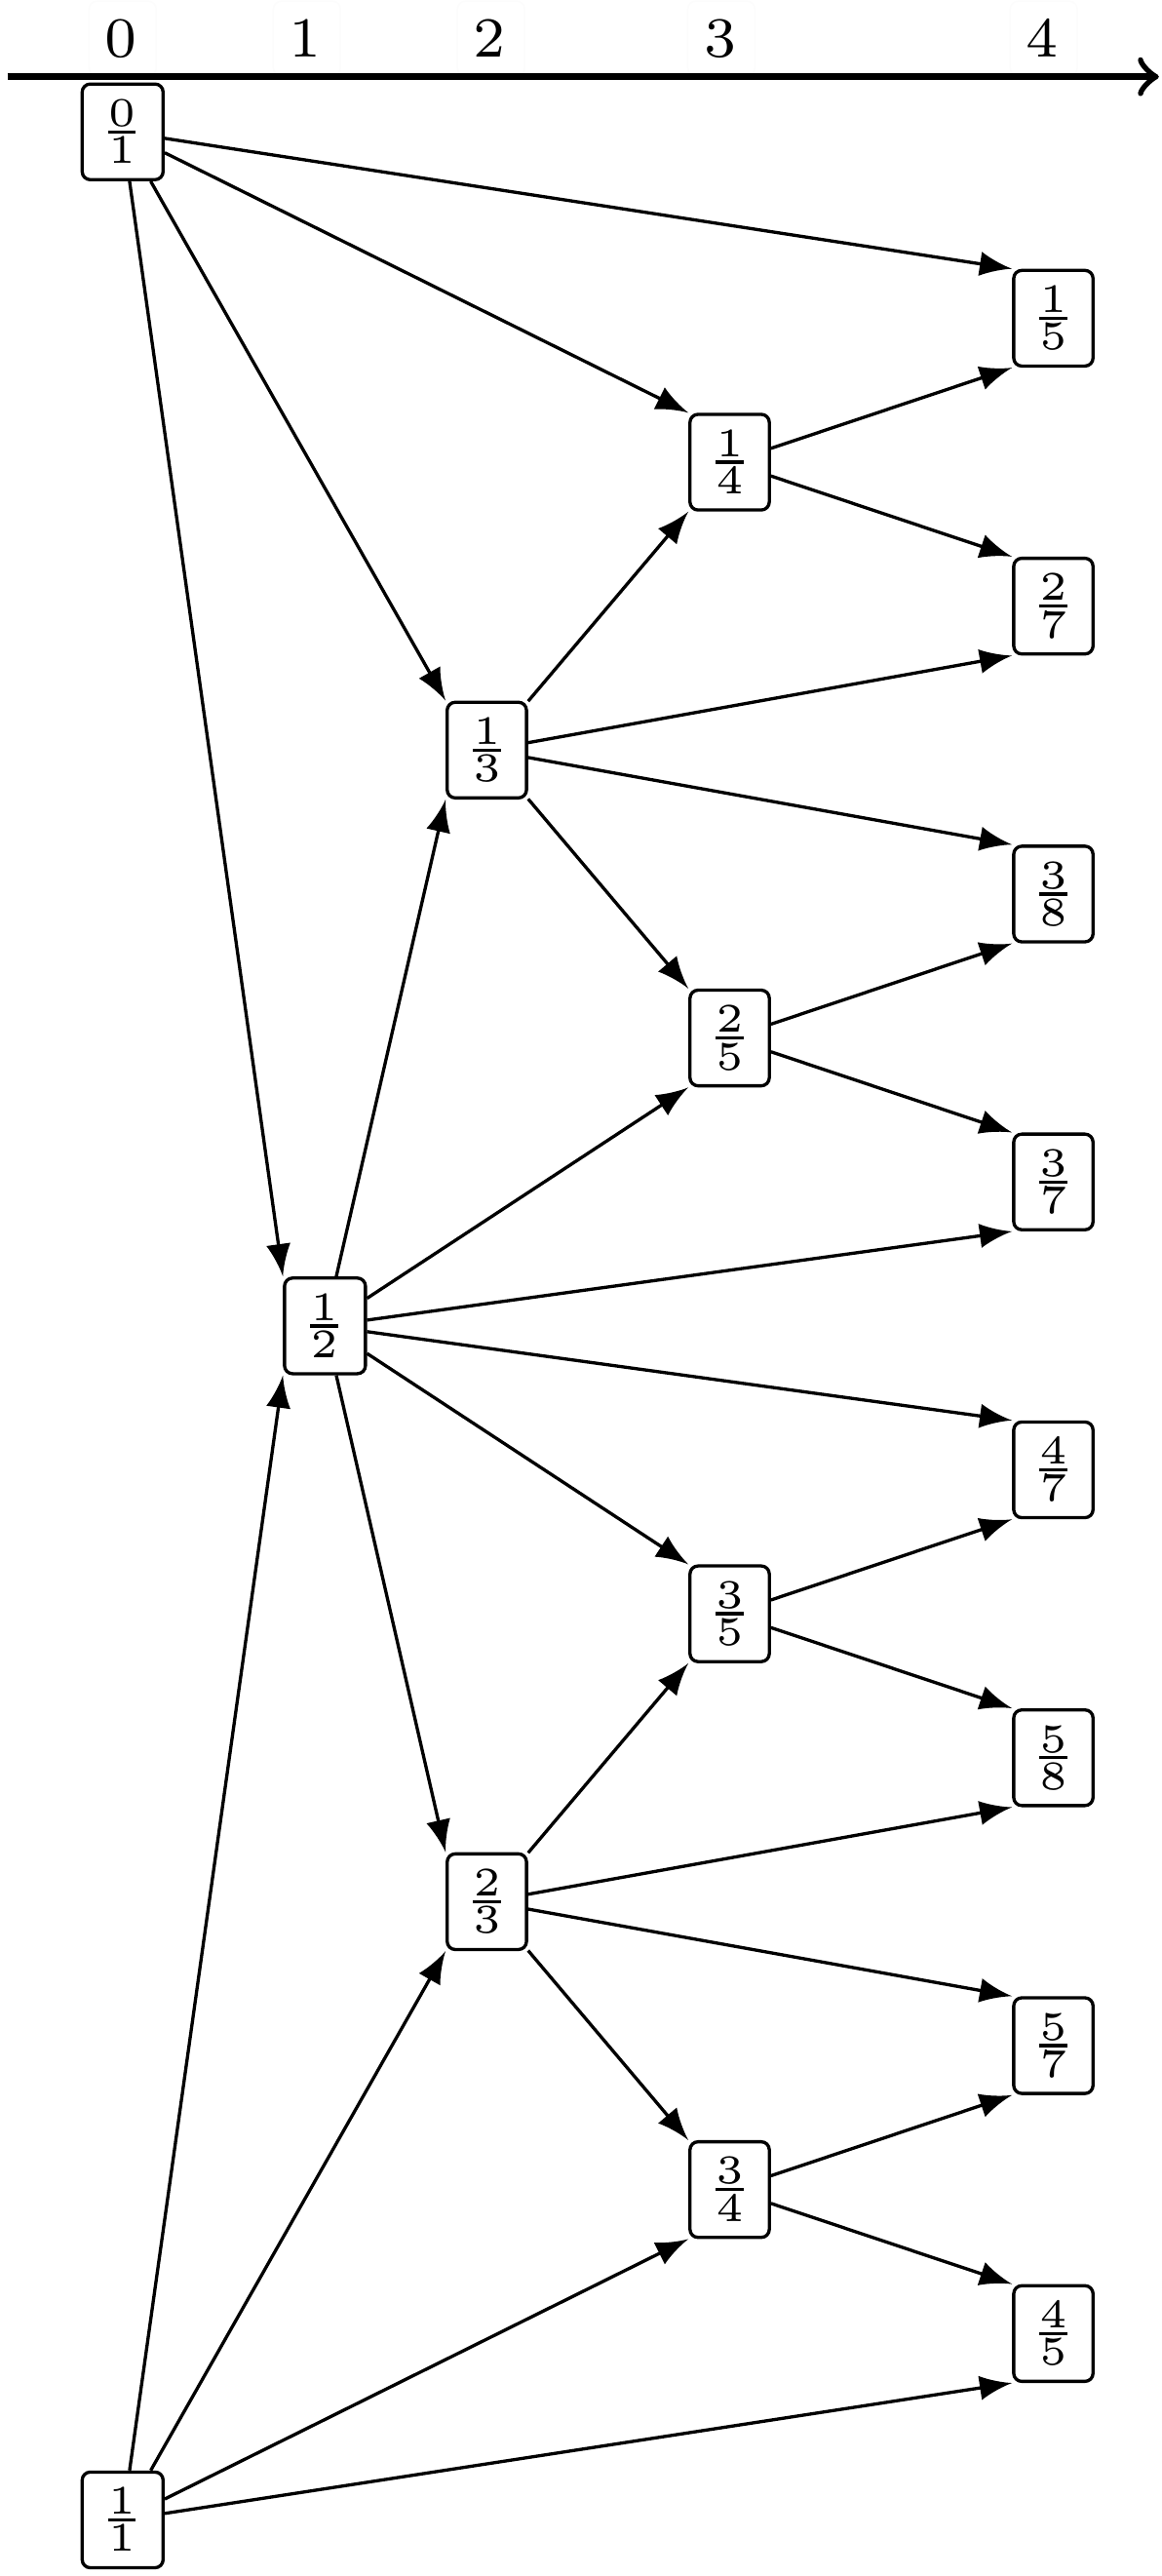
\includegraphics[width=\textwidth]{../../Report/Figures/FareyTrees/LR_RotNum/adding.png}
			\end{figure}
		\end{column}
	\end{columns}
\end{frame}

\begin{frame}{Farey-trees with Symbolic Sequences}
	\begin{columns}
		\begin{column}{.5 \textwidth}
			\begin{itemize}
				\item Keep the structure of the tree
				\item Replace starting nodes with symbolic sequences
				\item Use concatenation instead of farey-addition $\oplus$
			\end{itemize}
		\end{column}
		\begin{column}{.3 \textwidth}
			\vspace{-3em}
			\begin{figure}
				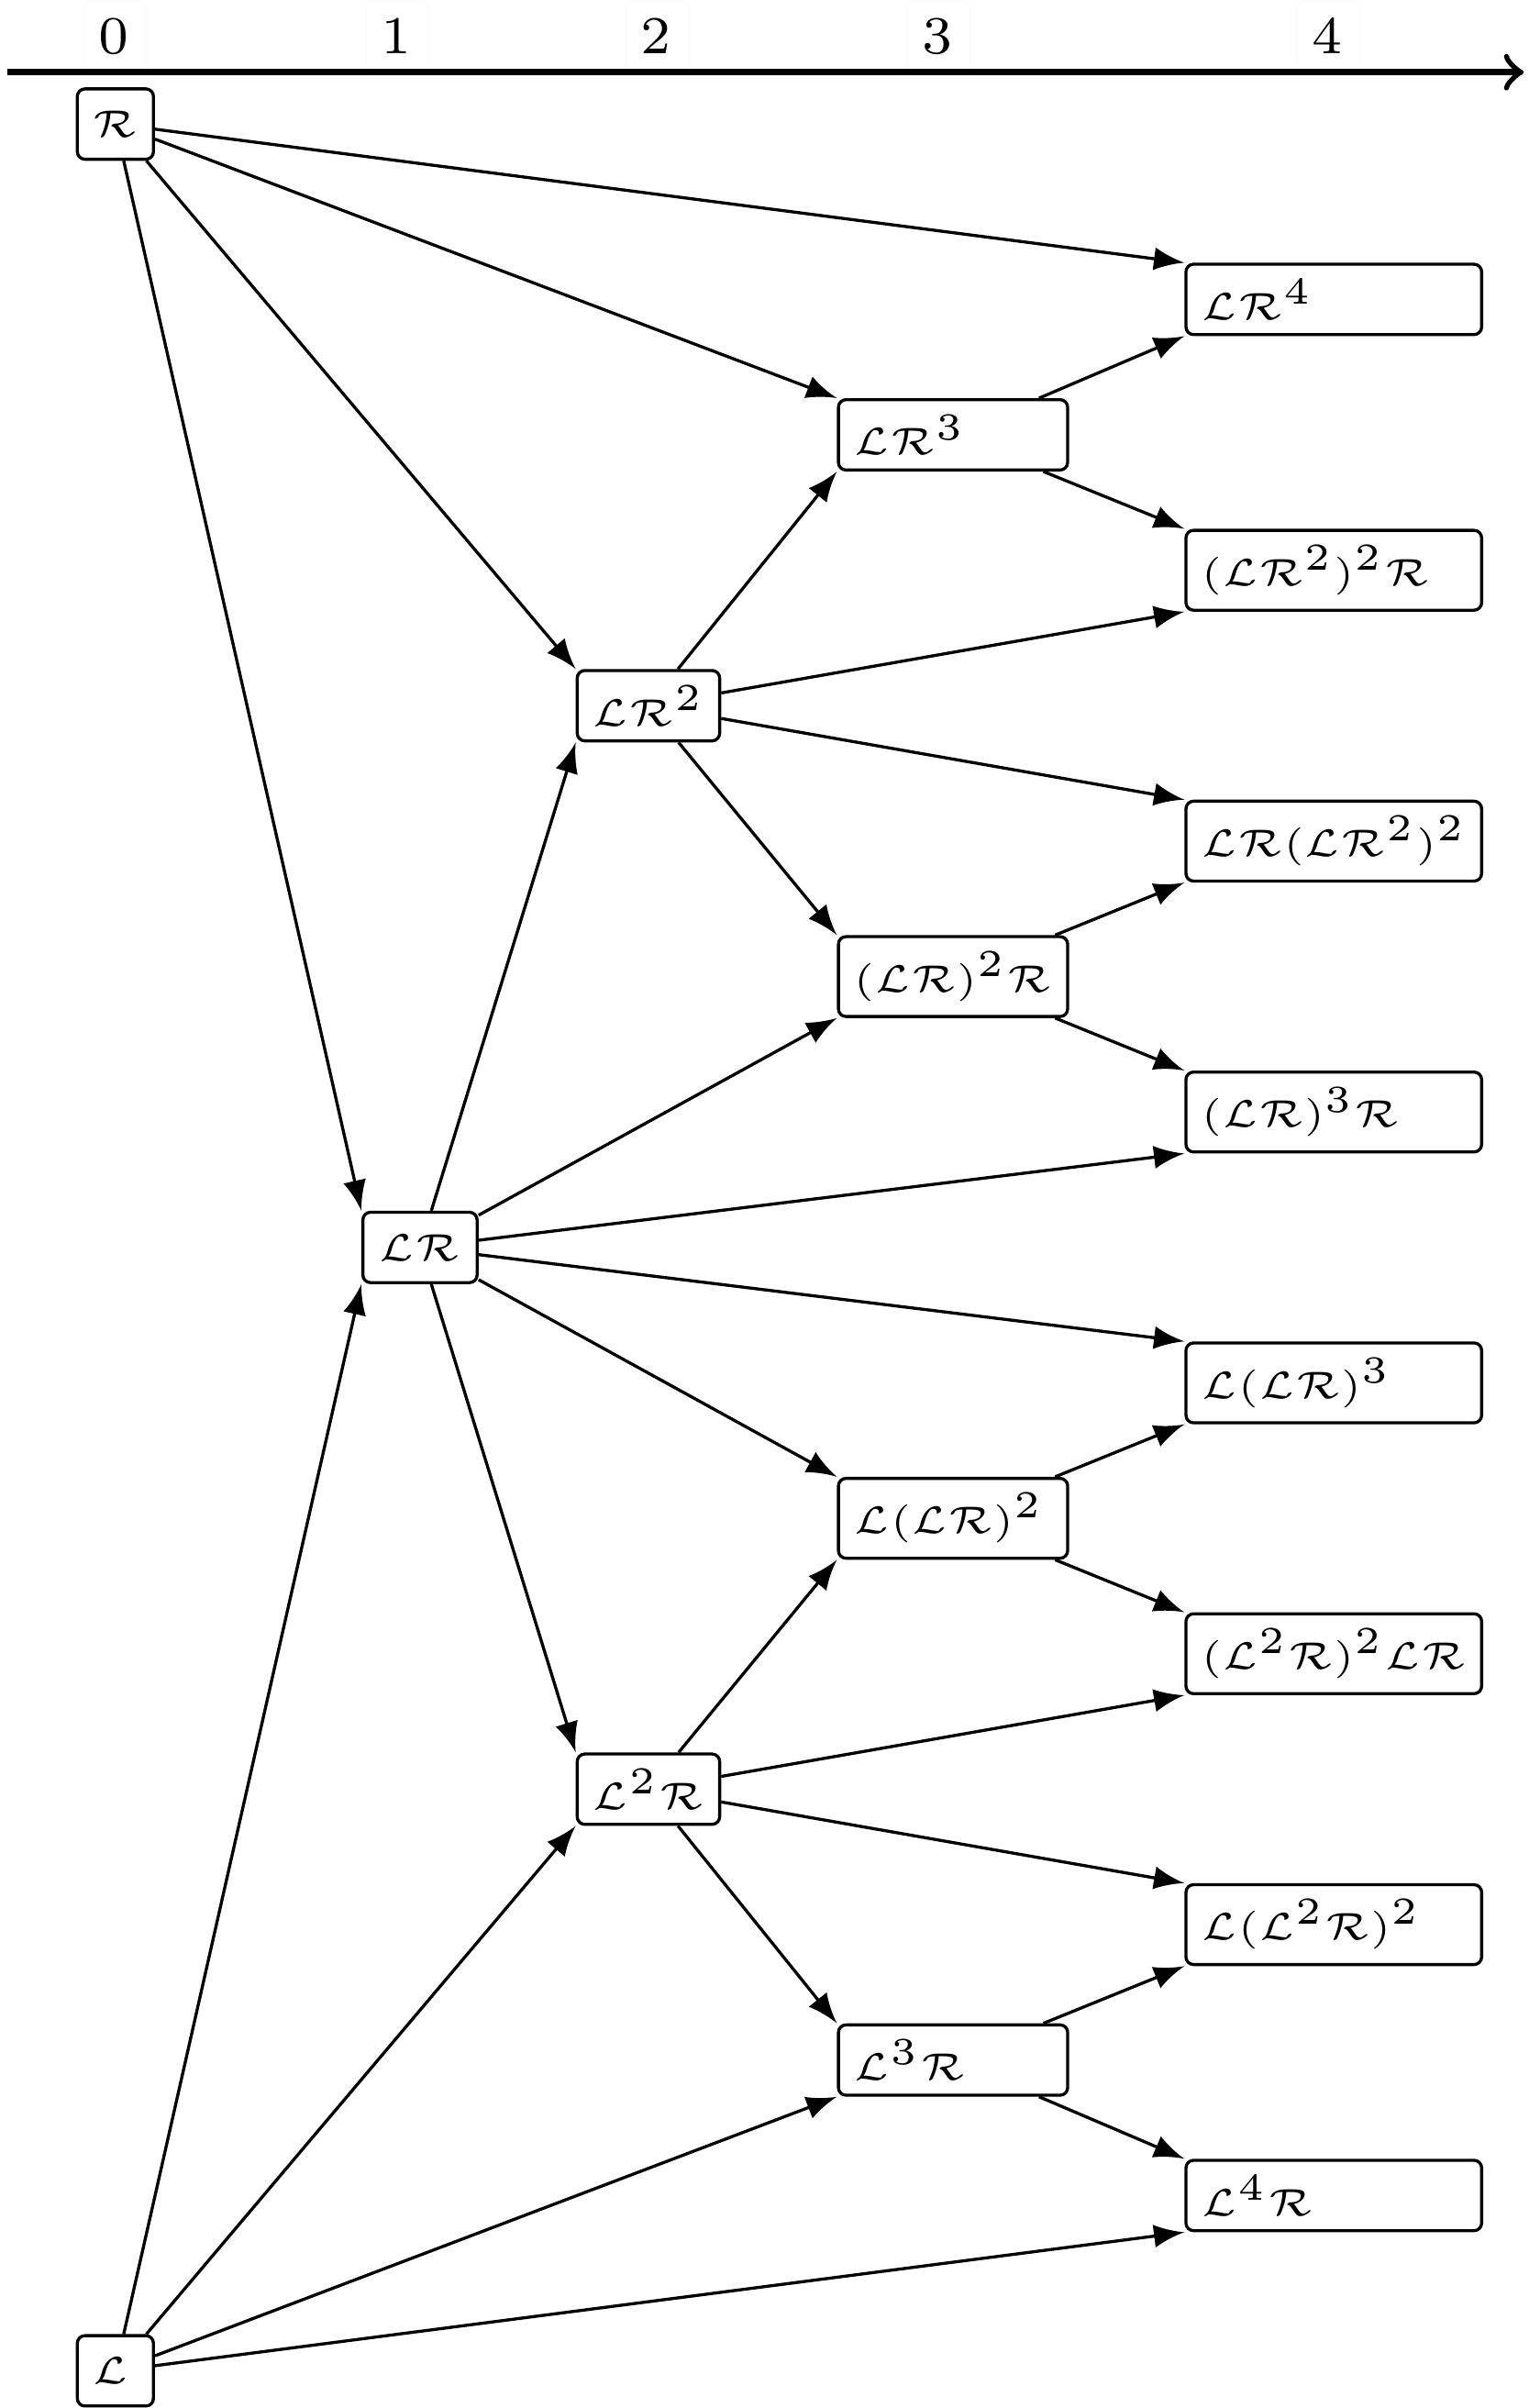
\includegraphics[width=\textwidth]{../../Report/Figures/FareyTrees/LR/adding.png}
			\end{figure}
		\end{column}
	\end{columns}
\end{frame}

\begin{frame}{Rotation Numbers}
	\vspace{-1em}
	\begin{definition}[Rotation Numbers]
		For a cycle $\sigma$ in a model with two branches $\L$ and $\R$, its rotation number is defined as the number of symbols $\L$ in its symbolic sequence divided by its period.
		This fraction is not to be reduced.
		\begin{align*}
			\dfrac{|\sigma|_\L}{|\sigma|}
		\end{align*}
	\end{definition}
	\pause
	\begin{definition}[Poincaré Rotaion Numbers]
		The original definition of Poincaré was the number of rotations divided by the period.
		For our purposes, the definition above works too and is easier to compute from symbolic sequences.
	\end{definition}
\end{frame}

\begin{frame}{Rotation Numbers}
	\begin{theorem}
		In both cases will the rotation number of two concatenated cycles $\rho(\sigma\varrho)$ be the farey-sum of the rotation numbers of the individual cycles $\rho(\sigma)$ and $\rho(\varrho)$.
		\begin{align*}
			\rho(\sigma\varrho) = \rho(\sigma) \oplus \rho(\varrho)
		\end{align*}
	\end{theorem}
	\pause
	Note that the denominator is the period of the cycles.
	They get added together in the farey-addition.

	\vspace{1em}
	\pause
	This is exactly what happens in period-adding structures.
\end{frame}

\begin{frame}{Period Adding in Between Chains}
	\vspace{-1em}
	Period-adding is common in between chains of cycles with the same period
	\begin{figure}
		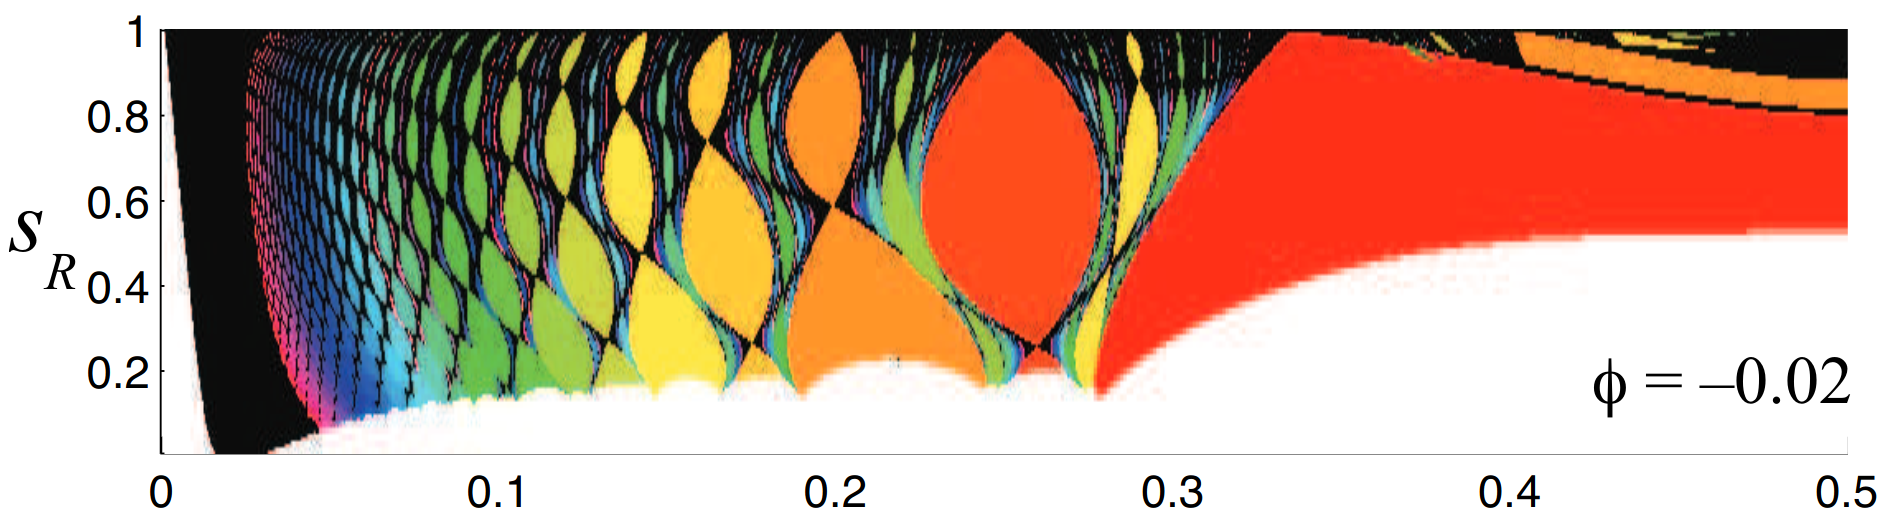
\includegraphics[width=.5 \textwidth]{Figs/tounge_adding.png}\\
		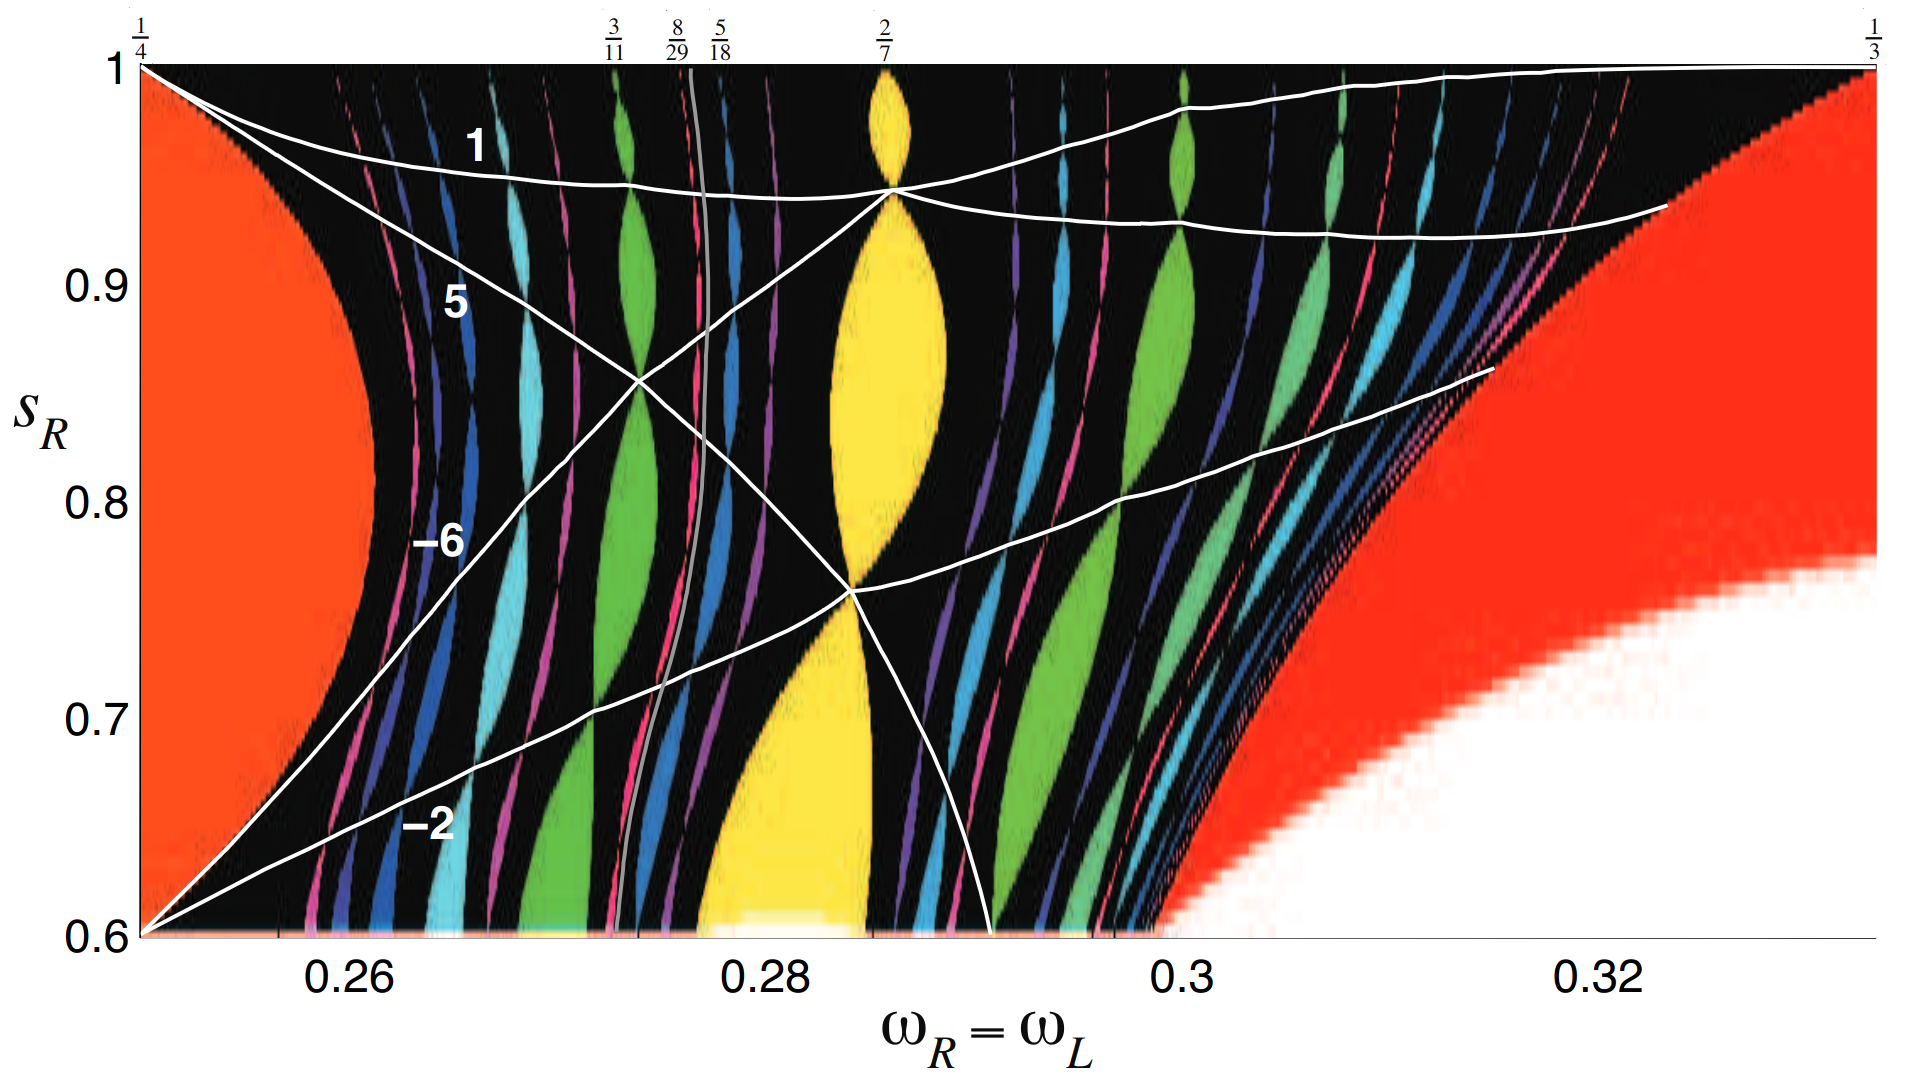
\includegraphics[width=.5 \textwidth]{Figs/tounge_adding_zoomed.png}
	\end{figure}
	\vspace{-2em}
	\begin{flushright}
		Pictures from \cite{simpson2010}
	\end{flushright}
\end{frame}
